\documentclass[12pt]{article}\pagestyle{myheadings}
\usepackage{graphicx}
\usepackage{placeins}

\textwidth 7.0 truein
\oddsidemargin -0.25in   %left-hand edge
\evensidemargin -0.5 truein  %right-hand edge
\topmargin -0.85in      %top of paper to top of head, pulls whole unit
\textheight 9.5in

%Enter your last name, the portfolio problem number, and the draft number.
\title{Homework 1 \\ Chaotic Dynamics - CSCI 4446}
\author{Denis Kazakov}
\date{January 17, 2015}


\usepackage{amsmath,amssymb,amsthm,amsfonts,graphicx}
%The following commands allow us to typeset theorems, propositions, definitions, etc.
\theoremstyle{plain}
\newtheorem{theorem}{Theorem}
\newtheorem{lemma}[theorem]{Lemma}
\newtheorem{corollary}[theorem]{Corollary}
\newtheorem{proposition}[theorem]{Proposition}
\newtheorem*{definition}{Definition}

\renewcommand{\qedsymbol}{\ensuremath{\blacksquare}}
\newcommand{\N}{\mathbb{N}}
\newcommand{\Z}{\mathbb{Z}}
\newcommand{\Q}{\mathbb{Q}}
\newcommand{\R}{\mathbb{R}}
\newcommand{\C}{\mathbb{C}} 

\begin{document}
\maketitle


\section{Problem 3}
\subsection{Chaotic Behaviour}

We can see on the Figure 1 that a slight change in initial population ratio ($0.2$ vs $0.20001$) results in different model path as time progresses. Therefore, we conclude that our system is extremely sensitive to initial conditions and is thus chaotic. 

\begin{figure}[h!]
\centering
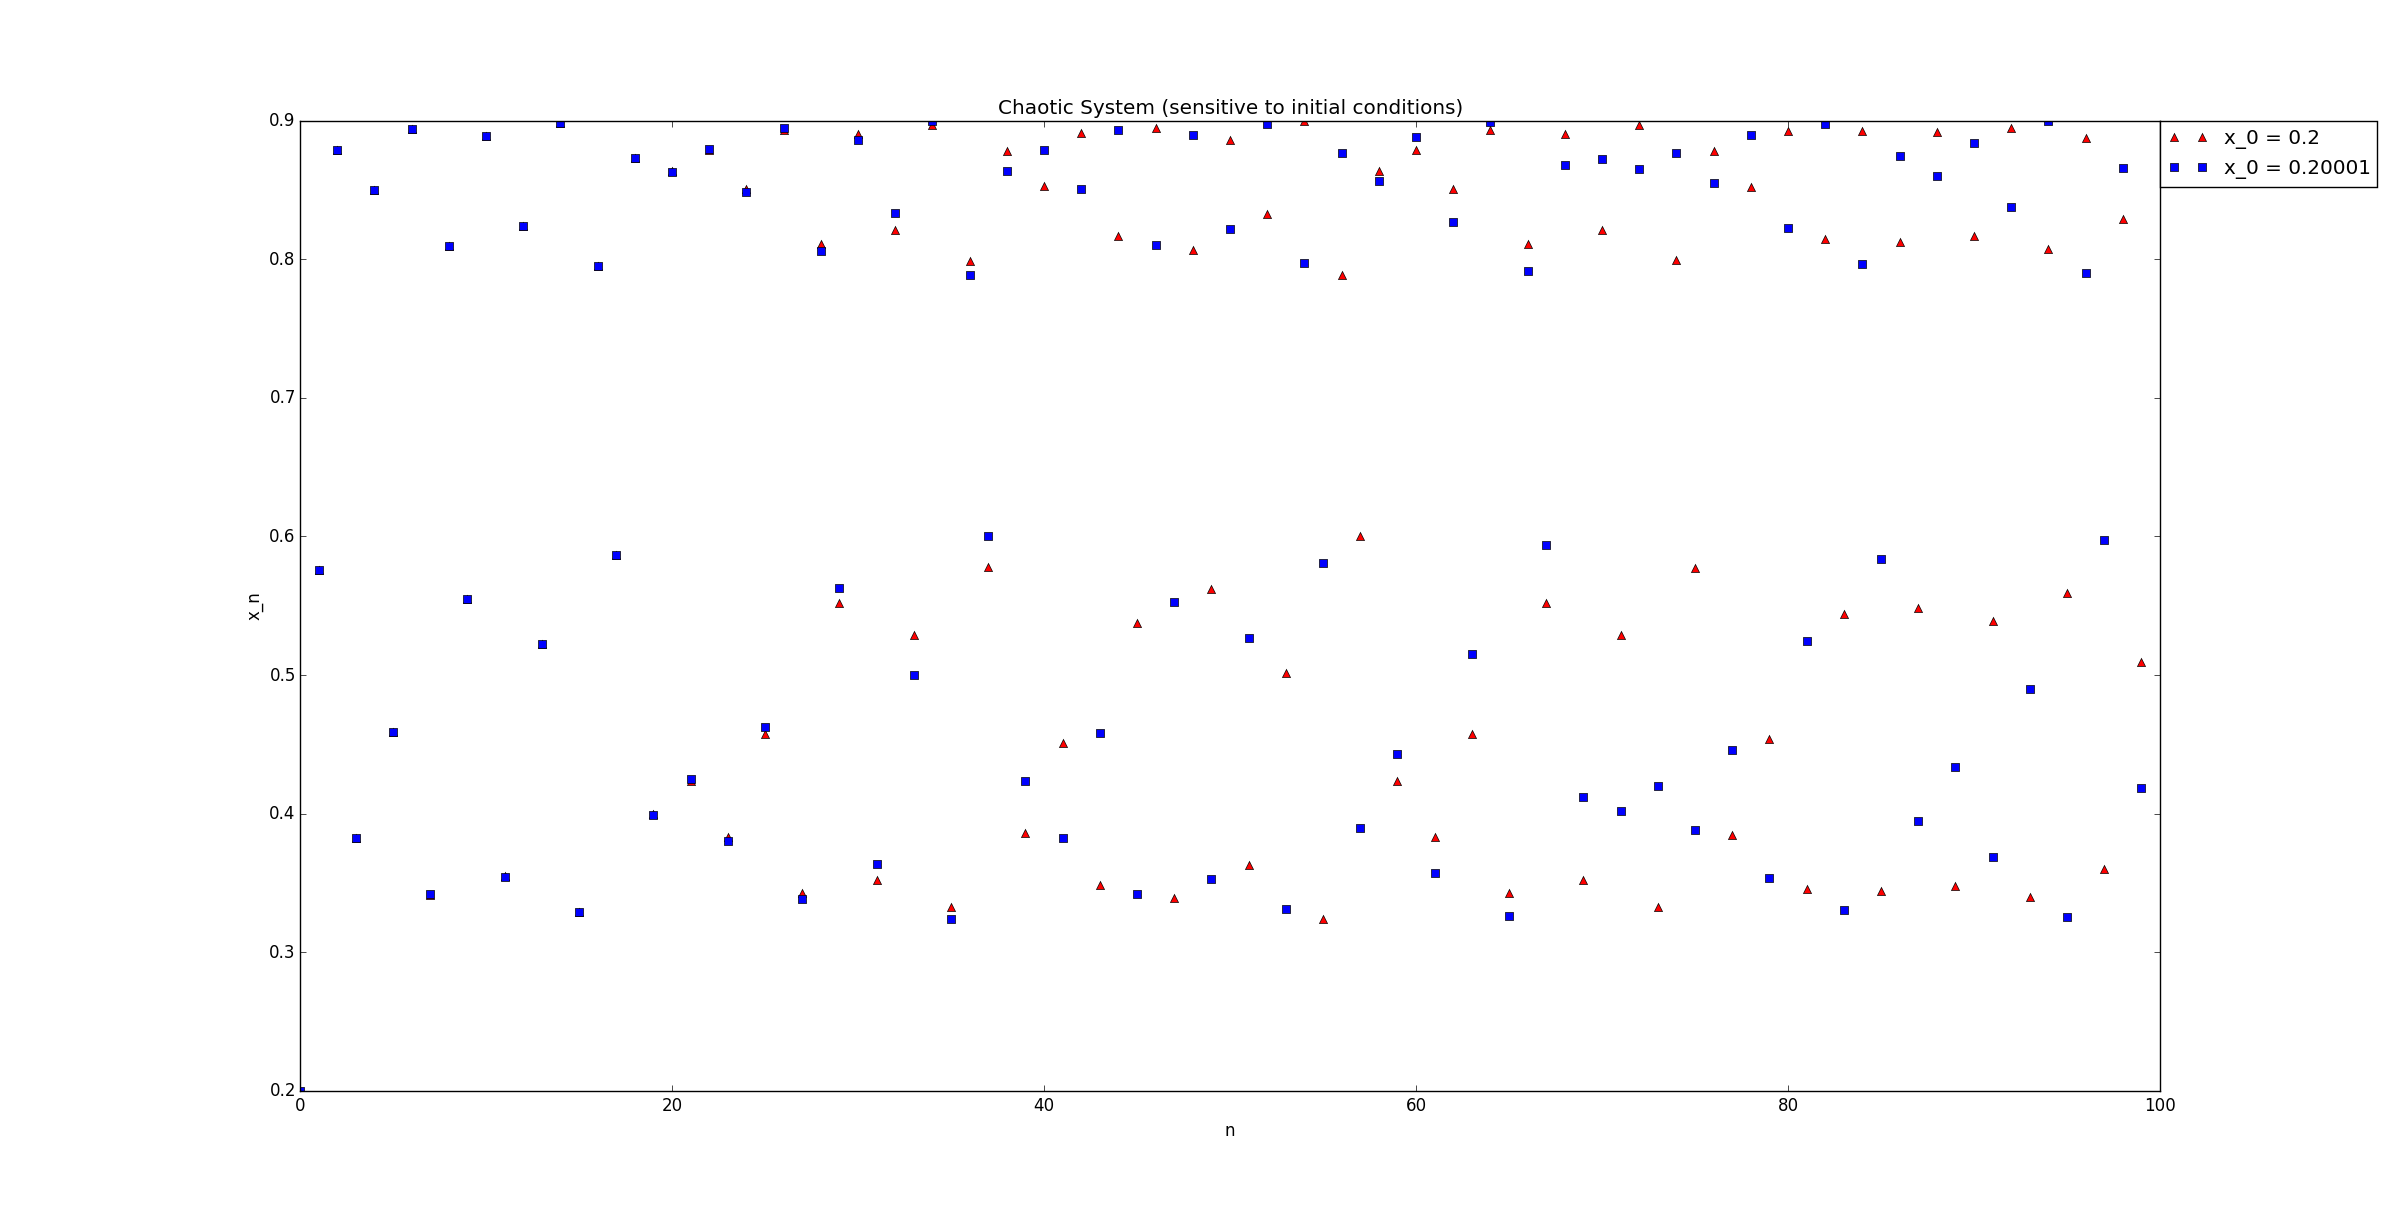
\includegraphics[scale=.3]{chaos}
\caption{Chaotic Behaviour (R=3.6, n=100, $x_0$ = 0.2 and 0.20001)}
\label{fig:my_label}
\end{figure}

\clearpage
\subsection{periodic behaviour}

I liked the conditions of $R=3.83$ because of its interesting oscillating (3-cycle period) behaviour that is very obvious on $x_n$ vs. $n$ graph, but might be confusing on $x_{n+1}$ vs. $x_n$ or $x_{n+2}$ vs. $x_n$, because those graphs weren't meant to capture a 3 periodic oscillation. However,once we plot $x_{n+3}$ vs. $x_n$, we clearly see how our line $y=x$ intersects the data points in exactly 3 locations, therefore showing that the system has "converged" to the 3-cycling periodic behaviour. 

	
\begin{figure}[h!]
\centering
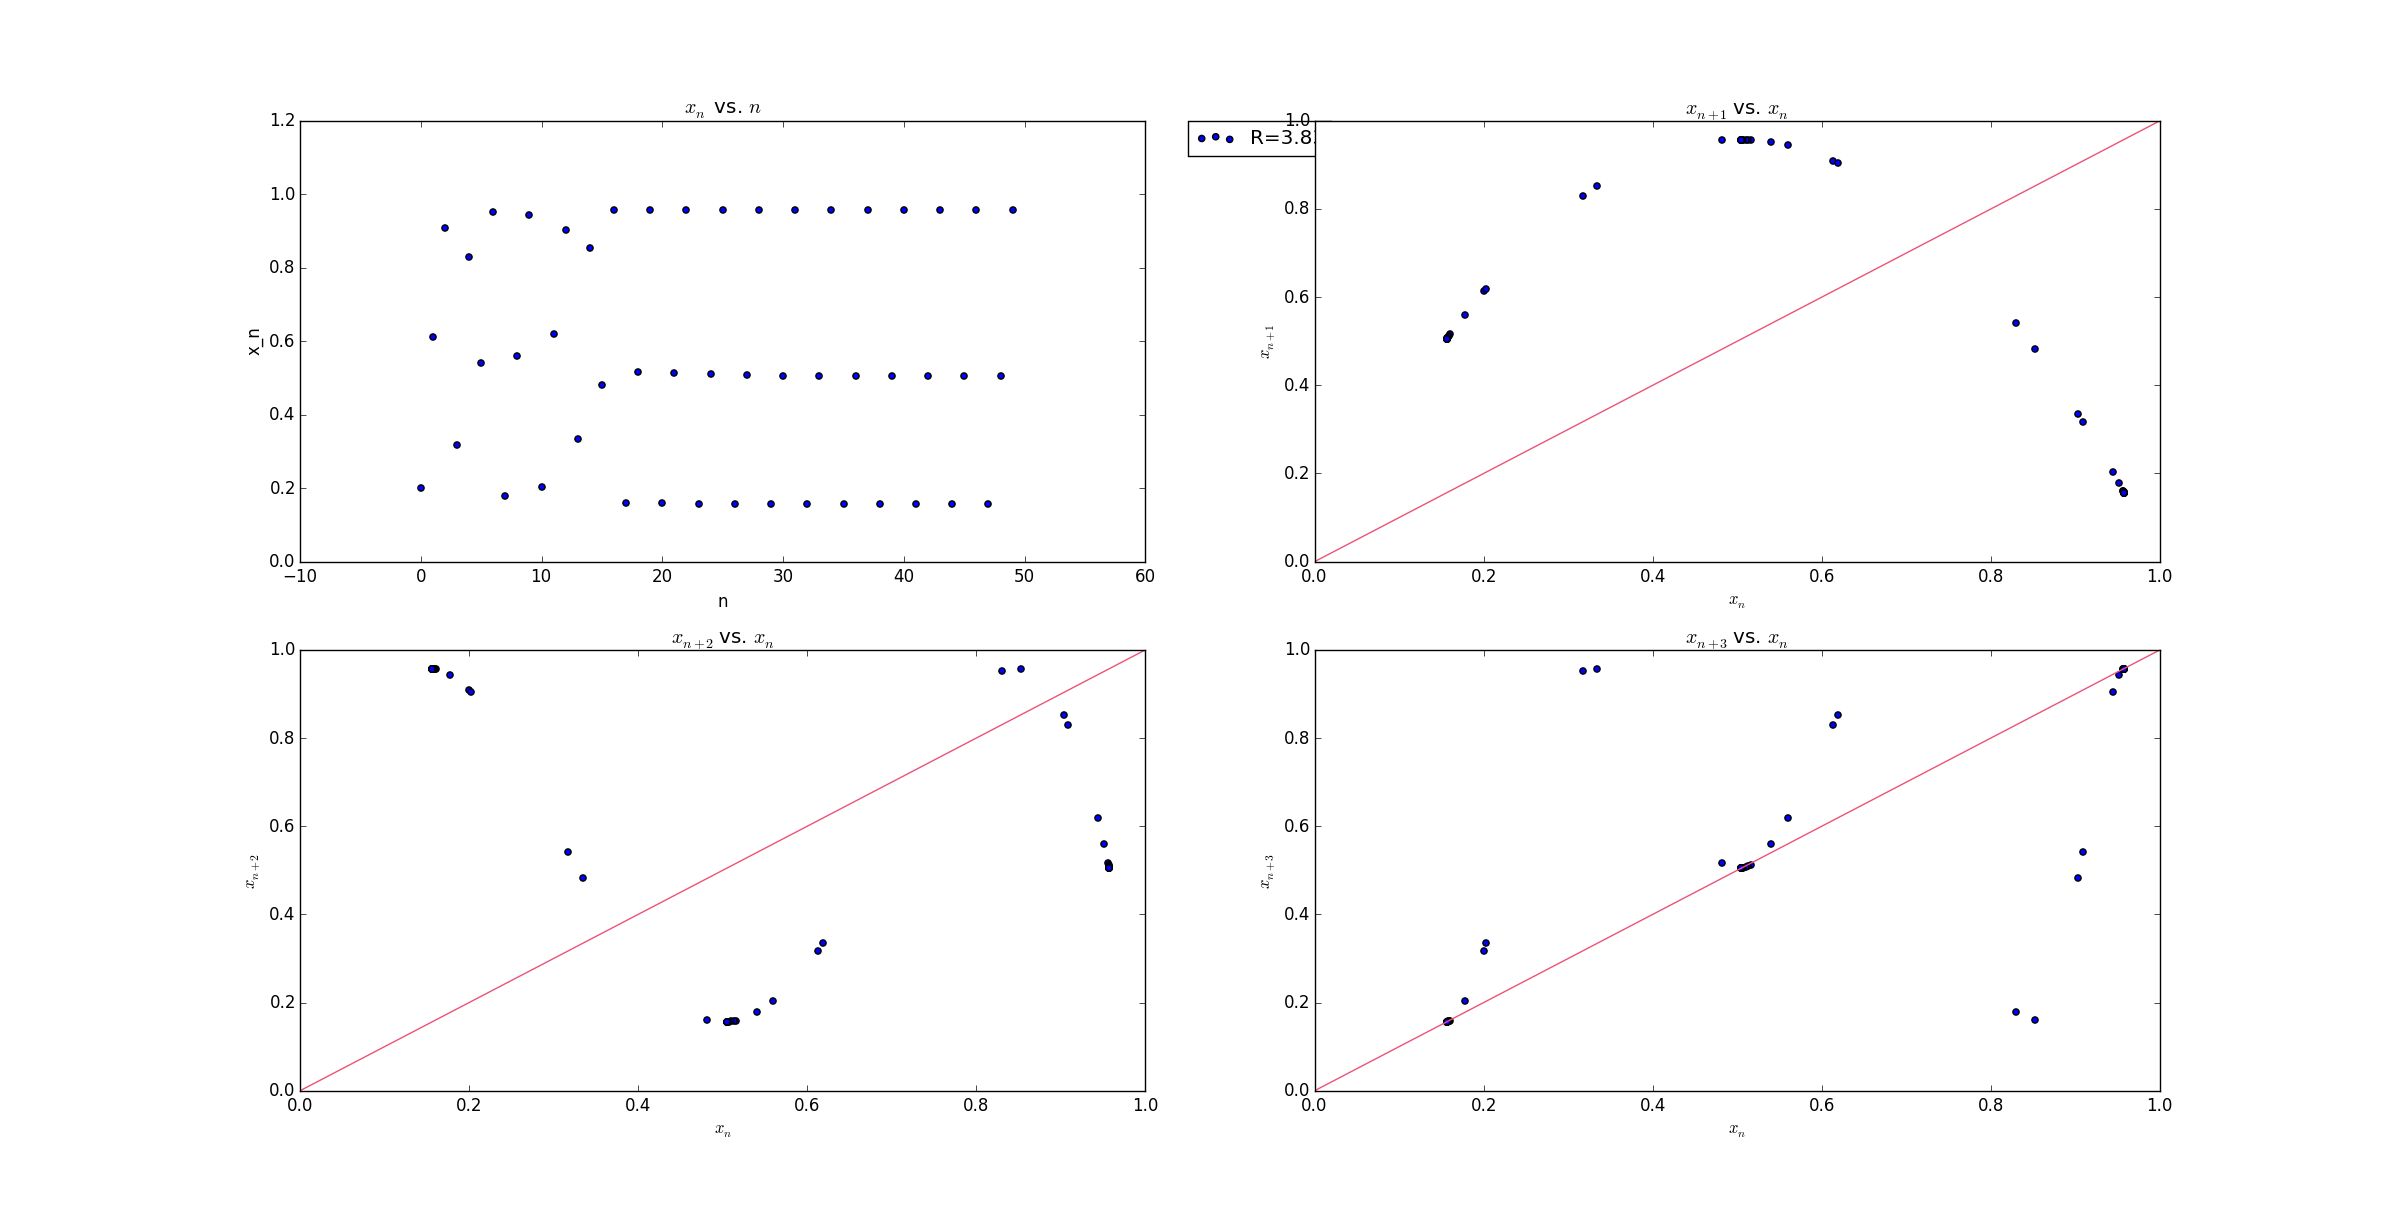
\includegraphics[scale=.3]{3,83.png}
\caption{periodic behaviour (R=3.83)}
\label{fig:my_label}
\end{figure}

	
\clearpage
\subsection{unstable fixed point}
Another condition I found interesting is $R=3.6$. I tried to set initial condition to that of a 2-cycling oscillation - $x_0 =0.86955$. Even though a clear 2-cycling behaviour didn't last long, it's interesting to note that the prediction was able to determine behaviour of the system for a brief period. 

\begin{figure}[h!]
\centering
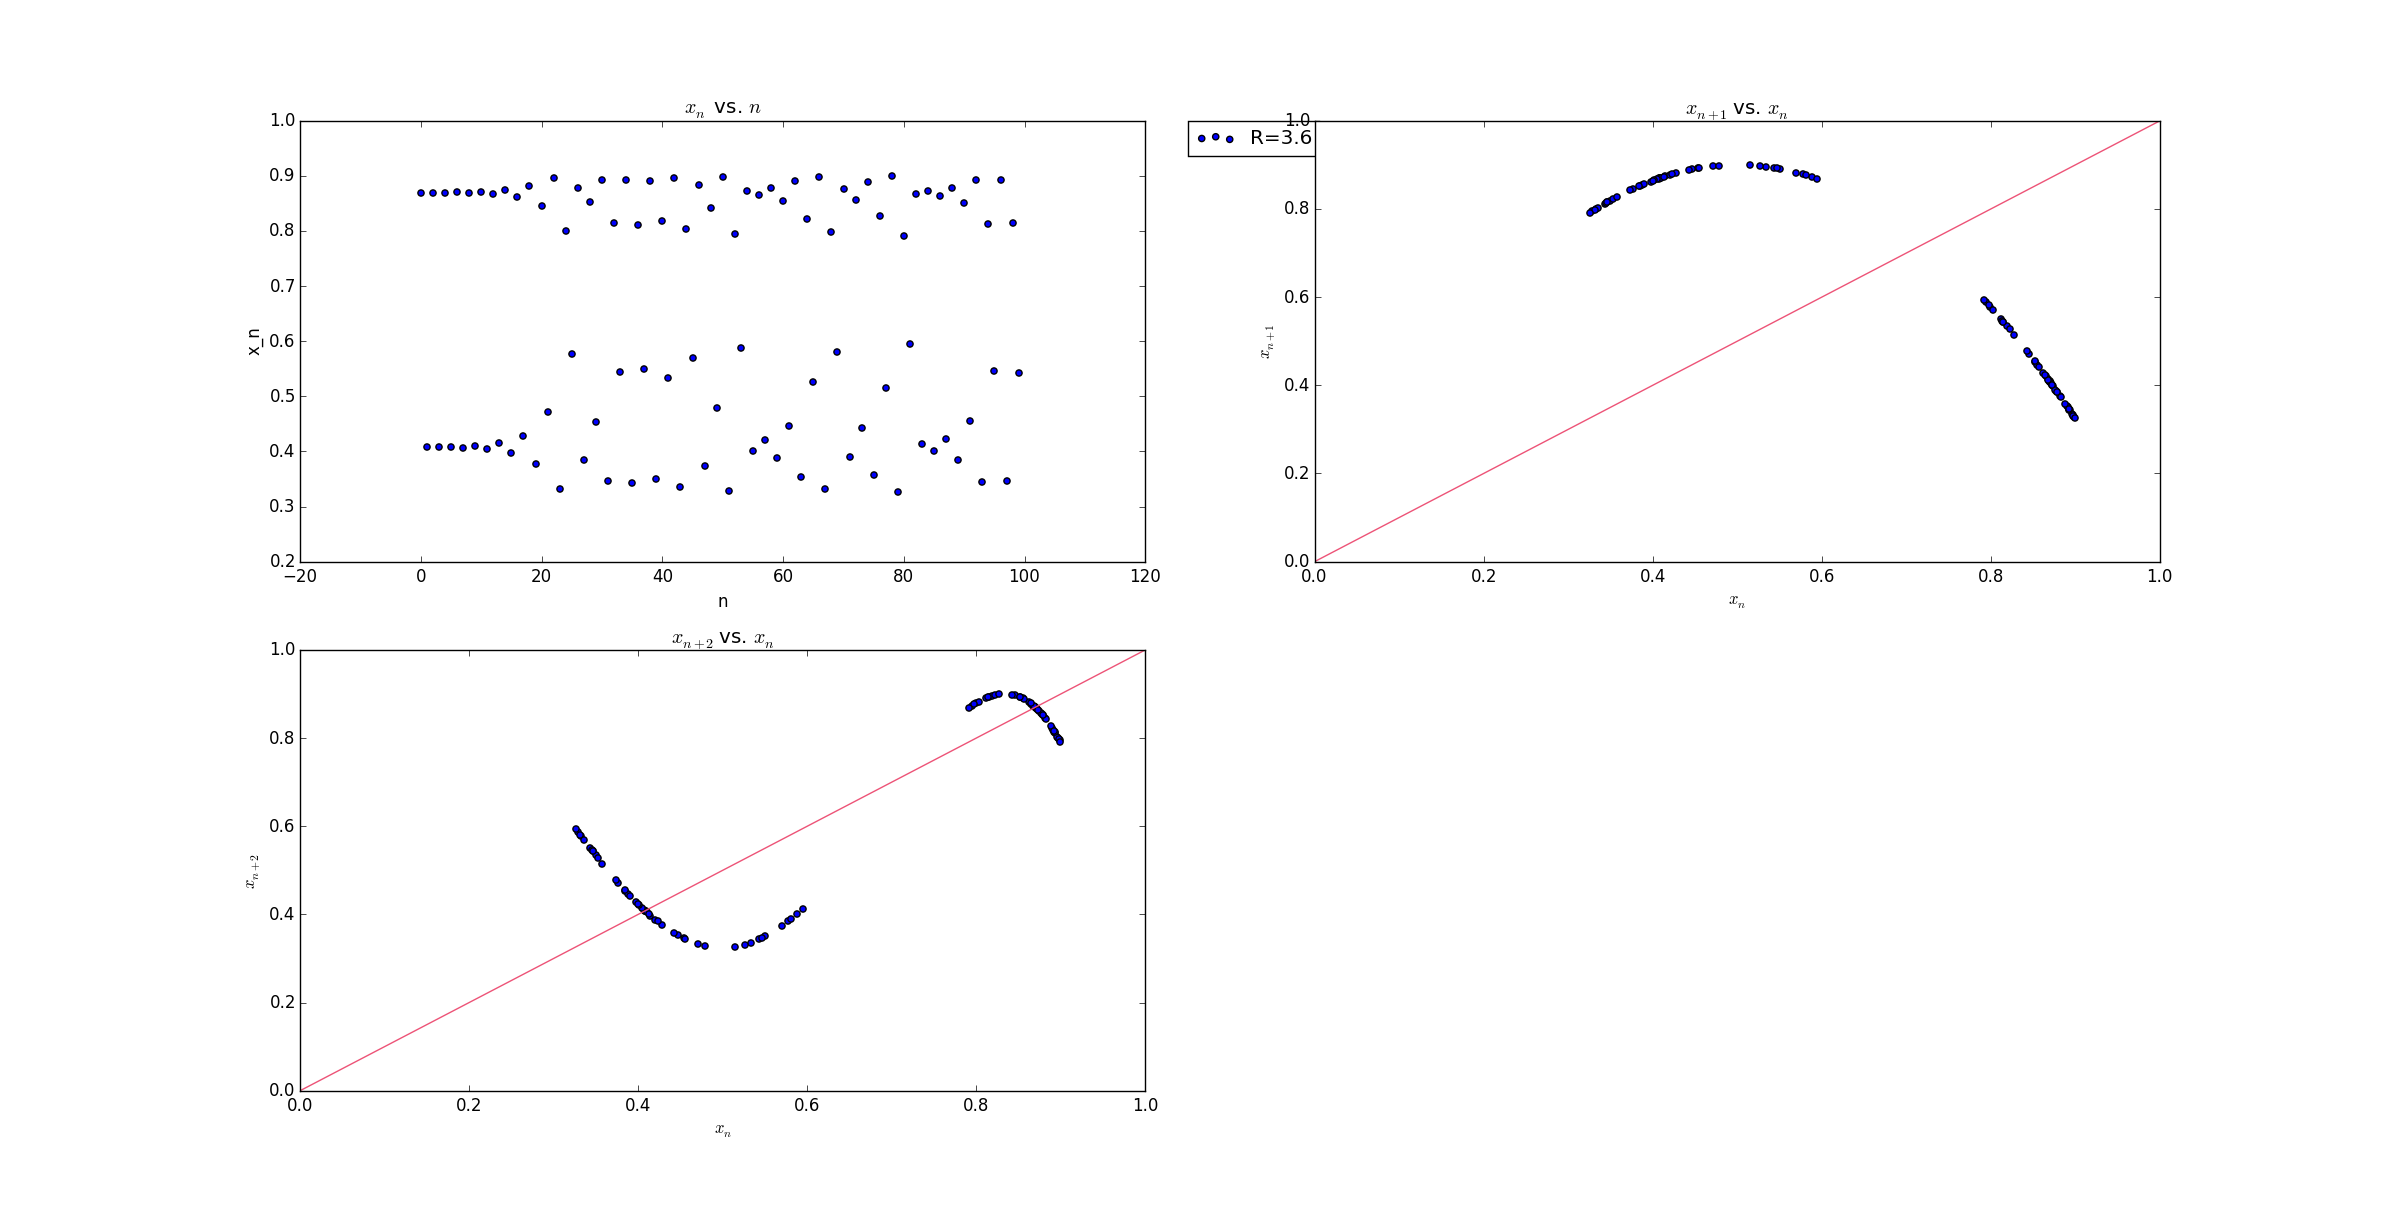
\includegraphics[scale=.2]{3,6.png}
\caption{unstable fixed point}
\label{fig:my_label}
\end{figure}

We can similarly force a fixed point, but because of the chosen R value, fixed point is unstable. 

\begin{figure}[h!]
\centering
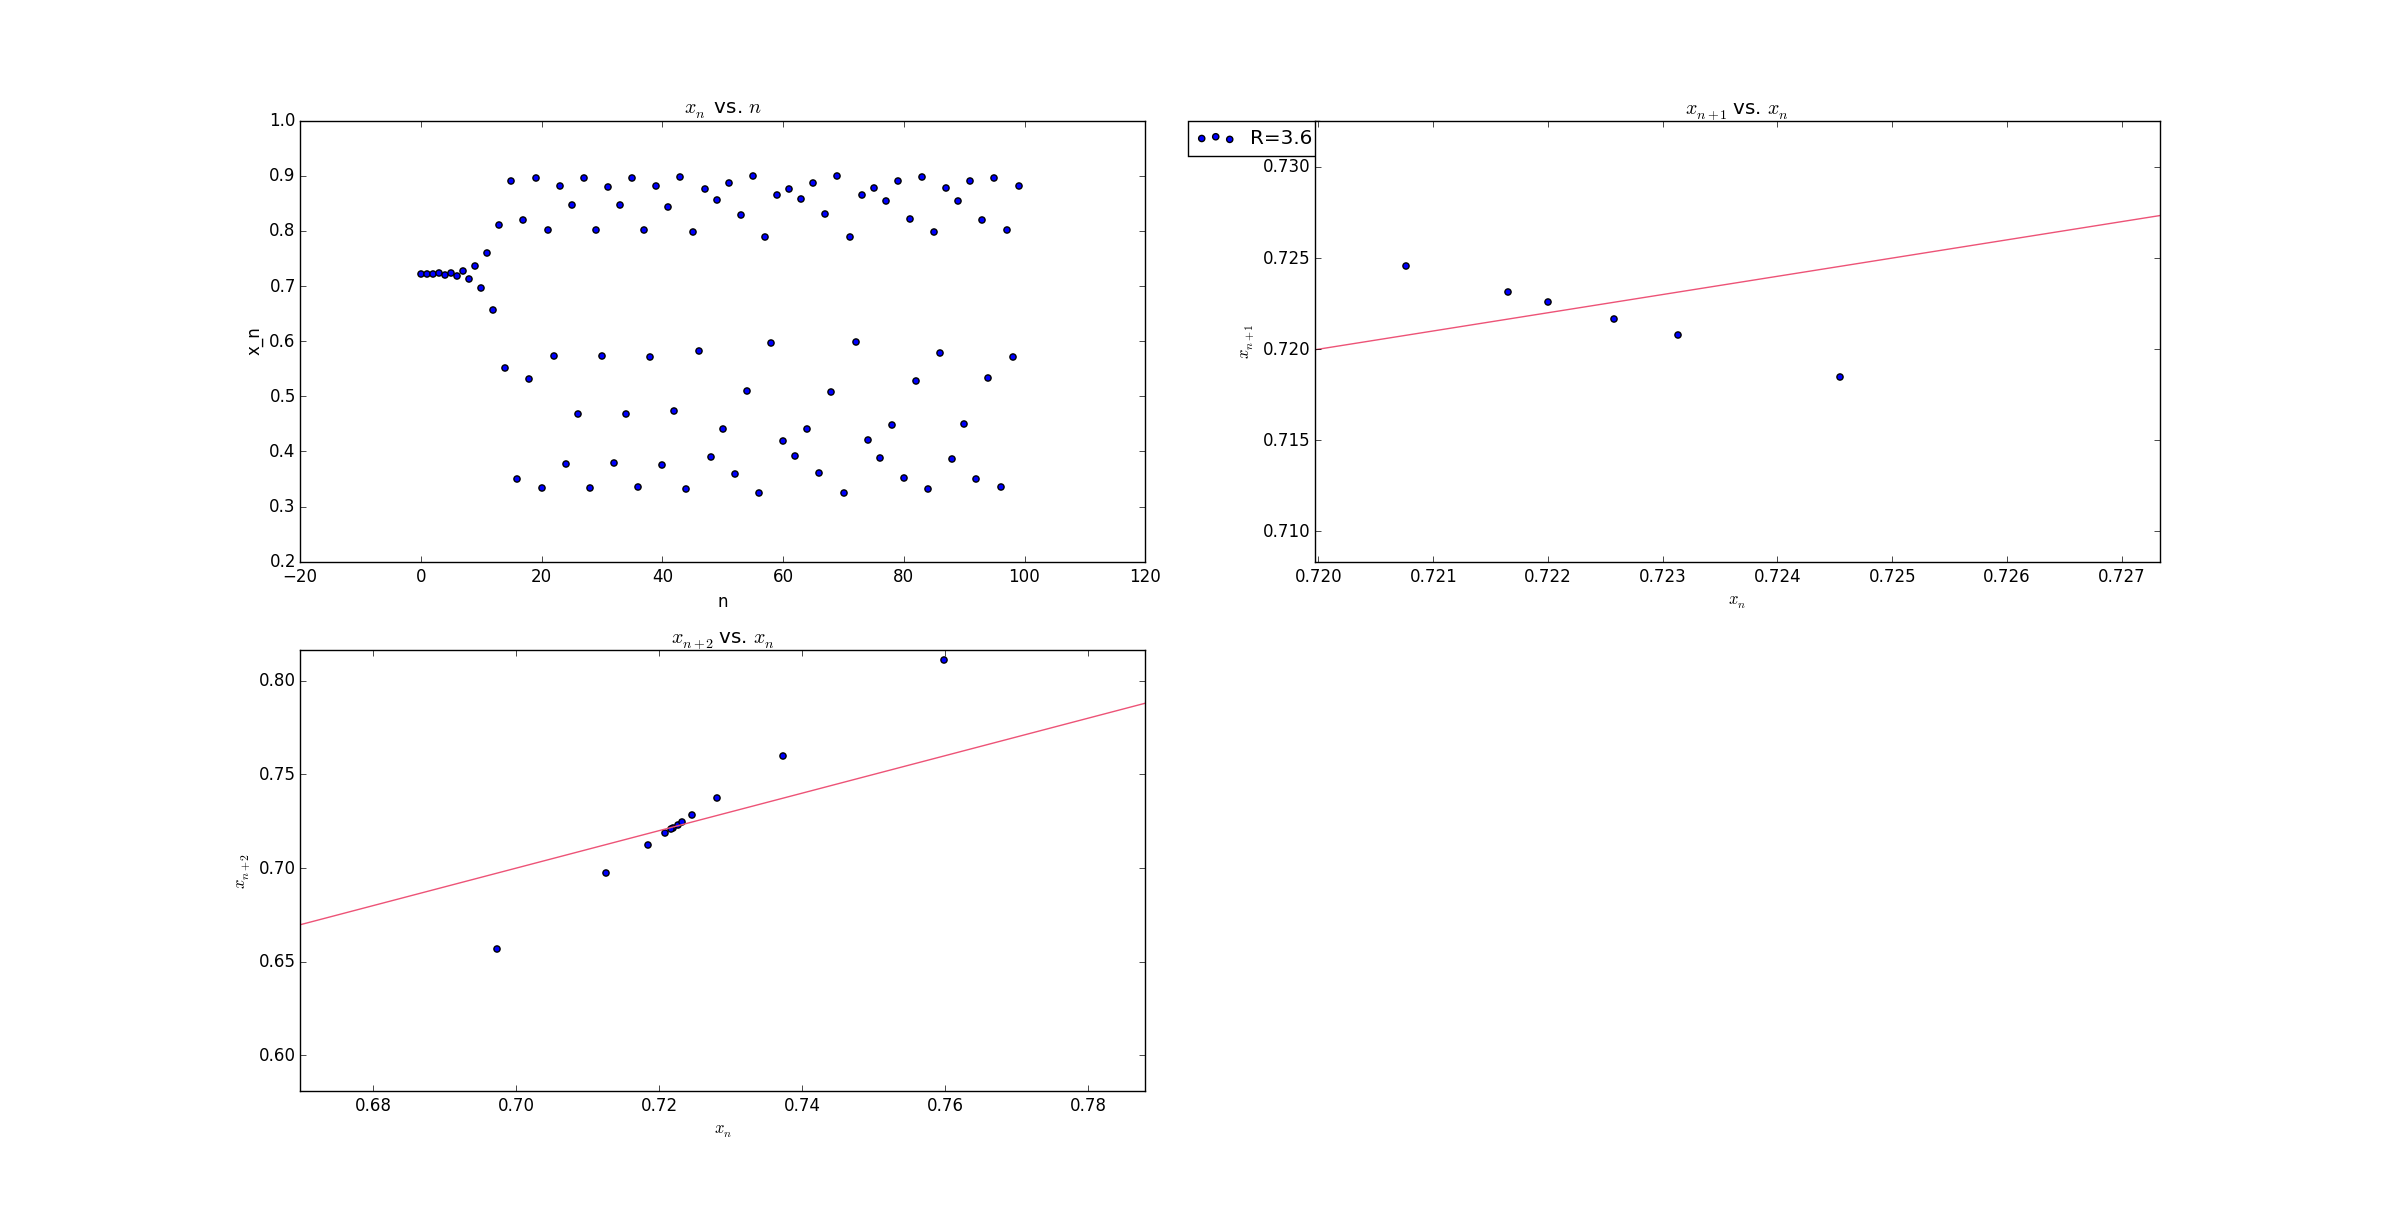
\includegraphics[scale=.2]{3,6-7223}
\caption{unstable fixed point}
\label{fig:my_label}
\end{figure}

\subsection{Questions}

As we set $R>4$, the system diverges and at some point, $x_0$ becomes greater than zero and that ruins our model. 

As we choose $R=2.5$, the system always converges towards the same fixed point as we change initial condition of $x_0$. Therefore, the system produces a stable fixed point attractor. 

\end{document}

